%
% Hello! Here's how this works:
%
% You edit the source code here on the left, and the preview on the
% right shows you the result within a few seconds.
%
% Bookmark this page and share the URL with your co-authors. They can
% edit at the same time!
%
% You can upload figures, bibliographies, custom classes and
% styles using the files menu.
%
% If you're new to LaTeX, the wikibook at
% http://en.wikibooks.org/wiki/LaTeX
% is a great place to start, and there are some examples in this
% document, too.
%
% We're still in beta. Please leave some feedback using the link at
% the top left of this page. Enjoy!
%
\documentclass[12pt]{article}

\usepackage[english]{babel}
\usepackage[utf8x]{inputenc}
\usepackage{amsmath}
\usepackage{graphicx}
\usepackage{cite}

\usepackage[normalem]{ulem}

\title{Computable Compressed Matrices\\Suplementary Material}
\author{Crysttian A. Paixão}

\bibliographystyle{plos2009}
\begin{document}
\maketitle

\begin{abstract}
Your abstract.
\end{abstract}

\section{Introduction}

In this supplementary material we will explore basic arithmetic operations
(addition, subtraction, division and multiplication) over the elements of
bitstring compressed arrays. We will consider integer matrices compressed via
both the SM and the VLB methods.

In these operations, the most important aspect is the bit-length of the result
in relation to those of the operands. As the operations are all done in
binary, when the result bit-length increases, the resulting matrix will require
more space to store and the operation in itself gets more complex, as in place
operations are not possible. In the following examples we will explore these
kinds of operations.

\subsection{Operations with Scalars}

\paragraph{Addition}

In base 2 the carry over  behavior is the same as we observer when operating
with decimals, only the base is different. Adding $1+1$ results in $0$ and a
carry over of 1, this is similar to the decimal sum $5+5$ where we also have a
carry over of 1. Other single digit additions in base 2 are: $1 + 0
= 1$, $0 + 1 = 1$, and $0 + 0 = 0$. Consider the following addition $n_1+n_2$
where $n_1=7$ and $n_2=10$. This addition is illustrated in table \ref{tab:01}
in both decimal and binary. Note that when we add $1+1$, a carry over is
generated to be added to bit on the left. In total we generate three bits in
carry over.

In Table \ref{tab:02} we show the addition of $7 + 7$ which generates a 4 bits
long number. In integer additions, the results may, in the very least, be as
long (in bits) as the greatest operand (for example $1+2=3$), but is frequently
longer.

\begin{table}[ht]
	\centering
    \caption{Comparing binary and decimal sum ($7+10$).}
    \begin{tabular}{crrrc}
    \hline
    	  & Decimal & & Binary & bit-length \\
    \hline      
    Carry Over& 	& & \textit{11100} & \\
    $n_1$ & 7   & & 111 & 3 \\
    $n_2$ & \underline{10}	& & \underline{1010} & 4 \\
    Total & 17	& & 10001 & 5 \\
    \hline
	\end{tabular}
    \label{tab:01}
\end{table}

\begin{table}[ht]
	\centering
    \caption{Comparacao da soma em base decimal e binaria.}
    \begin{tabular}{crrrc}
    \hline
    	  & Decimal & & Binario & Bit-length \\
    \hline      
    Carry & 	& & \textit{1110} & \\
    $n_1$ & 7   & & 111 & 3 \\
    $n_1$ & \underline{~7}	& & \underline{111} & 3 \\
    Total & 14	& & 1110 & 4 \\
    \hline
	\end{tabular}
    \label{tab:02}
\end{table}

\paragraph{Subtraction}
Depending of the number involved in this operation, the result may be negative.
This fact alone generates the need for an extra bit to represent the sign($+$ or
$-$). The usual way to achieve this is to use the  two's complement
\cite{flores1963logic} representation which has the advantage of making the
addition subtraction and multiplication operation the same as those for unsigned
binary numbers. To exemplify let's subtract $7$ from $10$. To make use of the
same algorithm of the sum we represent the operation as $10+(-7)$. First we
need to convert the operands to two's complement representation (C2):

\begin{itemize}
    \item The numbers will require an extra bit in C2. Thus 7 which is 3
bits long in binary, will require 4 bits in C2. As $7$ will be added to $10$,
the operands must be represented by 5 bits (4 bits to represent 10 plus one for
the signal). Therefore $7$ becomes $00111$ (in one's complement).

    \item Now the bits in 7 are flipped, going from $00111$ to $11000$.

    \item to the flipped number we add 1: $11000+1=11001$, which is the C2
representation of $-7$
\end{itemize}

Once completed the conversion, we add the numbers (see table  \ref{tab:03}).
Both operands require 5 bits because of C2. Most importantly, the left most
bit generated by the carry over, is discarded. That happens because to operate
in C2, the operands must have the same bit-length so any overflow in the result
must be discarded.

This operation would be possible without the use of C2 representation as 10 is
greater than 7 (see table \ref{tab:04} for this).

\begin{table}[ht]
	\centering
    \caption{Two's complement addition(subtraction) in decimal and binary.}
    \begin{tabular}{crrrc}
    \hline
    	  & Decimal & & C2 Binary & Bit-length \\
    \hline      
    Carry over & 	& & \textit{110000} & \\
    $n_2$ & 10	& & 01010 & 5 \\
    $+(-n_1)$ & \underline{+(-7)} & & \underline{11001} & 5 \\
    Total & 3	& & \sout{1}00011 & 5 \\
    \hline
	\end{tabular}
    \label{tab:03}
\end{table}

\begin{table}[ht]
	\centering
    \caption{Standard binary subtraction.}
    \begin{tabular}{crrrc}
    \hline
    	  & Decimal & & Binary & Bit-length \\
    \hline      
    Carry over& 	& & \textit{0111} & \\
    $n_2$ & 10	& & 1010 & 4 \\
    $-n_1$ & \underline{-7} & & \underline{111} & 3 \\
    Total & 3	& & 11 & 2\\
    \hline
	\end{tabular}
    \label{tab:04}
\end{table}

In conclusion, in the worst case subtraction will require the same number of
bits of the greatest operand, regardless of the use of C2 representation. As an
example, consider the subtraction $7-1$ (table \ref{tab:05}).

\begin{table}[ht]
	\centering
    \caption{Binary subtraction}
    \begin{tabular}{crrrc}
    \hline
    	  & Decimal & & Binary & Bit-length \\
    \hline      
    Carry over & 	& & \textit{000} & \\
    $n_1$ & 7	& & 111 & 3 \\
    $-n_3$ & \underline{-1} & & \underline{1} & 1 \\
    Total & 6	& & 110 & 3\\
    \hline
	\end{tabular}
    \label{tab:05}
\end{table}

\paragraph{Multiplication}
If multiplication is thought of as a series of sums, we can apply much the same
techniques. For example: $2 \times 3 = 3 + 3 = 2 + 2 + 2$. Table \ref{tab:06}
describes a simple multiplication.

\begin{table}[ht]
	\centering
    \caption{Binary Multiplication}
    \begin{tabular}{crrrc}
    \hline
    	  & Decimal & & Binary & Bit-length \\
    \hline      
    $n_2$ & 10	& & 1010 & 3 [VERIFICAR]\\
    $n_1$ & \underline{$\times 7$} & & \underline{111} & 1 \\
    & & & 1010  & \\
    & & & \underline{1010\ } & \\
    & & & $11110$ & \\
    & & & \underline{1010\ \ } & \\
    Total& 70 & & 1000110 & 7\\
    \hline
	\end{tabular}
    \label{tab:06}
\end{table}

In multiplication the behavior of the bit-length is different from the sum and
subtraction. In the worst case the product has a bit-length which is the sum of
the bit-lengths of the factors. For example, in the product $7\times7$, the
product is 6 bits long: $49$ which in binary is $110001$.

If a signed integer is involved in the multiplication, we need to use C2
representation. To illustrate this case let's calculate $10\times-7$. in C2,
this opration becomes $01010\times11001$. Table \ref{tab:07} contains the
details. The basic difference is that the sign bits (in bold), positioned to
the left, are not involved in the operation. Only in the end they are used to
determine the sign of the product: $0$ meaning positive and $1$ negative. In
the worst case the bit-length of the product is the sum of the bit-lengths of
the factors plus 1 due to the sign.


\begin{table}[ht]
	\centering
    \caption{Multiplication involving a signed integer.}
    \begin{tabular}{crrrc}
    \hline
    	  & Decimal & & Binary & Bit-length \\
    \hline      
    $n_2$ & 10	& & \textbf{0}1010 & 5 \\
    $\times -1n_1$ & \underline{$\times -7$} & & \underline{\textbf{1}1001} & 5
\\
    & & & 1010  & \\
    & & & \underline{0000\ } & \\
    & & & $01010$ & \\
    & & & \underline{0000\ \ } & \\
    & & & 001010 & \\
    & & & \underline{1010\ \ \ } & \\
    Total& -70 & & \textbf{1}1011010 & 8\\
    \hline
	\end{tabular}
    \label{tab:07}
\end{table}

\paragraph{Division}
Division, in contrast to multiplication, requires successive subtractions until
a remainder is reached which may or may not be zero. To illustrate the
procedure in binary, table \ref{tab:08} describes the division of $50$ by $10$.
Note the successive binary subtractions. The bit-length of the quotient is, in
the worst case, equal to the bit-length of the dividend when this is longer
than that of the divisor. With each subtraction, we add $1$ to the quotient
which is initially $0$. The process ends when the remainder is $0$ or less than
the divisor.

When the division involves a signed operand, we do the same as with the
multiplication, the operations is executed on the unsigned operands and the
sign is applied at the end.

\begin{table}[ht]
	\centering
    \caption{Binary division as a series of subtractions.}
    \begin{tabular}{crrrrr}
    \hline
    	  & Decimal & & Binary & Decimal quotient & Binary quotient\\
    \hline  
    $n_4$ & 50 					& & 110010
&0& 000 \\
    $n_2$ & \underline{-10} 	& & \underline{001010}  &\underline{+1}&
\underline{+001} \\
    Remainder & 40      			& & 101000
&1& 001
\\
    $n_2$ & \underline{-10} 	& & \underline{001010}  &\underline{+1}&
\underline{+001} \\
    Remainder & 30      			& & 011110
&2& 010
\\
    $n_2$ & \underline{-10} 	& & \underline{001010}  &\underline{+1}&
\underline{+001} \\
    Remainder & 20      			& & 010100
&3& 011
\\
    $n_2$ & \underline{-10} 	& & \underline{001010}  &\underline{+1}&
\underline{+001} \\
    Remainder & 10      			& & 001010
&4& 100
\\
    $n_2$ & \underline{-10} 	& & \underline{001010}  &\underline{+1}&
\underline{+001} \\
    Remainder & 0      				& & 000000
&5& 101 \\
    \hline
	\end{tabular}
    \label{tab:07}
\end{table}

So far we have examined the 4 fundamental arithmetic operations. In summary the
implication for memory allocation of the results are the folowing, in the worst
case scenarios:

\begin{itemize}
\item Addition: requires 1 extra bit above the bit-length of the greatest
operand;
\item Subtraction: Requires the same number of bits as the greatest
operand;
\item Multiplication: Requires the sum of the bit-lenghts of the
operands;
\item Division: Requires the same bit-length as the dividend;
\end{itemize}


When operating with signed integers, an extra bit is used for the sign.

The operations on single numbers (scalars) as exposed above are a simplification
of the
actual operations taking place on the bitstrings as we compute with compressed
matrices. Additional details will be provided below when we discuss the
operation with matrices. Note that we are restricting the example to operations
which generate integer results. Handling of float operations and compression
will be the subject of a subsequent paper.

\begin{figure}[h]
 \centering
 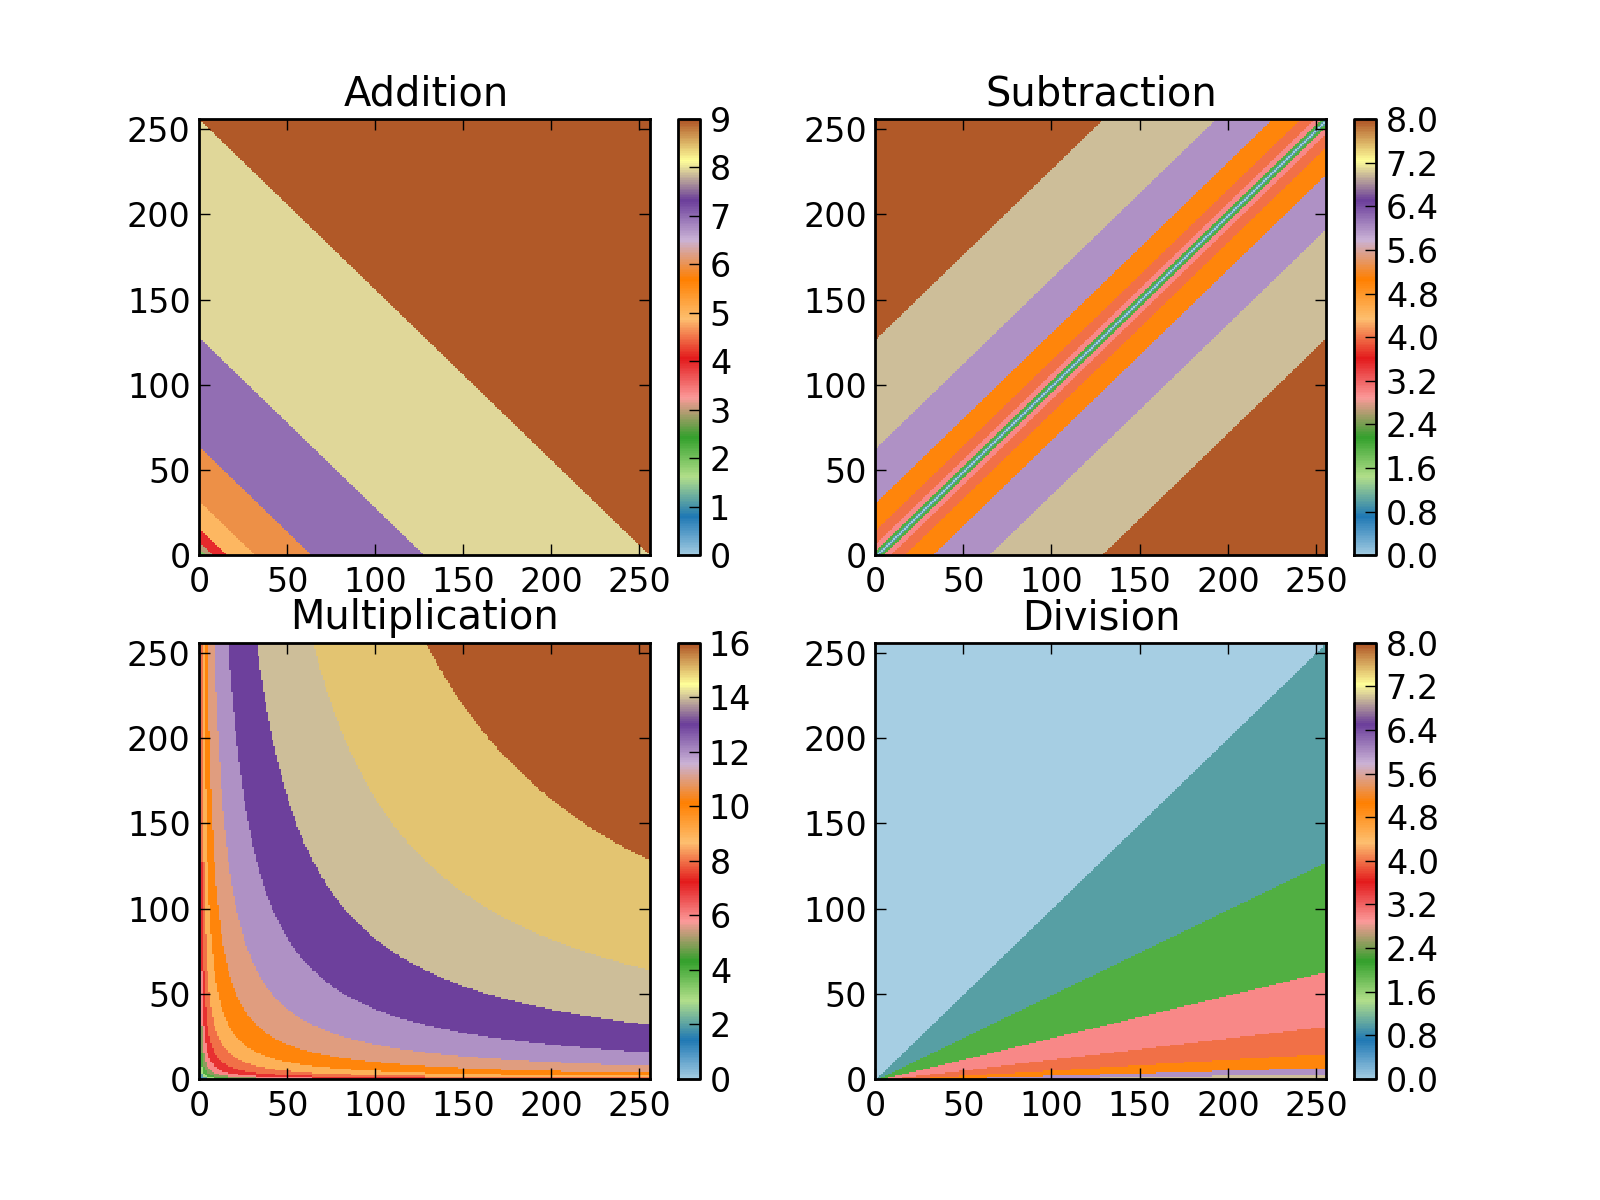
\includegraphics[width=12cm]{./bitlength.png}
 % simples.png: 4800x3600 pixel, 600dpi, 20.32x15.24 cm, bb=0 0 576 432
 \caption{bitlength of the results for each of the four operations. The axes
represent the values of the operands.}
 \label{fig:bitlength}
\end{figure}


\subsection{Operation on Bitstrings}

To illustrate operations with bitstrings, consider the matrices $A$ an $B$,
both $3 \times 4$:



\begin{equation}
	A = \begin{bmatrix}
			1 & 3 & 5 & 8\\ 
			12 &14  & 6 & 9\\ 
			3 & 7 & 10 & 11
		\end{bmatrix}
\end{equation}

e

\begin{equation}
	B = \begin{bmatrix}
			1  & 3  & 7 & 9\\ 
			1  &3   & 14 & 15\\ 
			20 & 30 & 2 & 1
		\end{bmatrix}
\end{equation}

After bitstring compression by the SM method, they become $3 \times 1$. They
are show in decimal and binary from in \ref{eq:01} and
\ref{eq:02}. The elements in $A$ and $B$ are 4 and 5 bits long, respectively
(the ``supreme minimum''). the ellipses ("$\ldots$") in the binary matrix
correspond the extra zeros to the left. Since the strings are written into 64
bits integers, sometimes we end up with unused bits to the left.

\begin{equation}\label{eq:01}
	AA = \begin{bmatrix}
			4952\\ 
			52841\\ 
			14251
		\end{bmatrix} 
        =
        \begin{bmatrix}
			\ldots0001001101011000\\ 
			\ldots1100111001101001\\ 
			\ldots0011011110101011
		\end{bmatrix}
        =
        \begin{bmatrix}
\ldots\underbrace{0001}_{1}\underbrace{0011}_{3}\underbrace{0101}_{5}\underbrace
{1000}_{8}\\
\ldots\underbrace{1100}_{12}\underbrace{1110}_{14}\underbrace{0110}_{6}
\underbrace{1001}_{9}\\ 
\ldots\underbrace{0011}_{3}\underbrace{0111}_{7}\underbrace{1010}_{10}
\underbrace{1011}_{11}
		\end{bmatrix}
\end{equation}

e

\begin{equation}\label{eq:02}
	BB = \begin{bmatrix}
			36073\\ 
			36303\\ 
			686145
		\end{bmatrix}
        =
         \begin{bmatrix}
			\ldots00001000110011101001\\ 
			\ldots00001000110111001111\\ 
			\ldots10100111100001000001
		\end{bmatrix}
        =
        \begin{bmatrix}

\ldots\underbrace{00001}_{1}\underbrace{00011}_{3}\underbrace{00111}_{7}
\underbrace{01001}_{59}\\
\ldots\underbrace{00001}_{1}\underbrace{00011}_{3}\underbrace{01110}_{14}
\underbrace{01111}_{15}\\
\ldots\underbrace{10100}_{20}\underbrace{11110}_{30}\underbrace{00010}_{2}
\underbrace{00001}_{1}
		\end{bmatrix}
\end{equation}

Consider now just the bitstring stored in the first line of each matrix ($AA$
and $BB$). To recover the original elements we need to now the bit-lengthof
the blocks of memory containing them, for the SM method they are all the same
length. To obtain the values in an efficient way, we will use a binary mask.
The mask will recover the first and third blocks at the same time to save time.
The mask is stored as a bitstring the same length as those storing the matrix
elements. The mask for the first and third elements of matrix $AA$ is depicted
in \ref{eq:06}. To recover the second and fouth elements, we apply the mask
shown on \ref{eq:07}. For Matrix $BB$, see \ref{eq:08} and \ref{eq:09} for the
respective masks.



\begin{equation}\label{eq:06}
\text{Matrix AA's mask for positions 1 and 3} = \ldots0000111100001111
\end{equation}

\begin{equation}\label{eq:07}
\text{Matrix AA's mask for positions 2 and 4} = \ldots1111000011110000
\end{equation}

\begin{equation}\label{eq:08}
\text{Matrix BB's mask for positions 1 and 3} = \ldots00000111110000011111
\end{equation}

\begin{equation}\label{eq:09}
\text{Matrix BB's mask for positions 2 and 4} = \ldots11111000001111100000
\end{equation}

Once defined the mask we can apply it to matrices $A$ and $B$. We use the mask
by applying the boolean function AND. Let tempA and tempB the recovered
elements. The recovering process is illustrated below. Note that only the
positions where the mask is $1$ are retained.

%\begin{equation}\label{eq:10}
  \begin{align*}
   A[1,1]			&=	\ldots0001|0011|0101|1000\\
   \text{mask A}	&=	\ldots0000|1111|0000|1111\\
   tempA 			&=	\ldots0000|0011|0000|1000
  \end{align*}
%\end{equation}

%\begin{equation}\label{eq:11}
  \begin{align*}
   B[1,1]			&= \ldots00001|00011|00111|01001 \\
   \text{mask B}	&= \ldots00000|11111|00000|11111 \\
   tempB 			&= \ldots00000|00011|00000|01001
  \end{align*}
%\end{equation}

\paragraph{Addition}

Suppose we want to add both matrices and store it in a matrix $S$. for that the
blocks of tempA and tempB must have the same length. As for the addition we
need, in the worst case, an extra bit, the block length of the resulting
bitstring will be 6. The string from each matrix, padded on the left towards
this new length,  are shown in equations \ref{eq:12} and \ref{eq:13}.

\begin{equation}\label{eq:12}
tempA =  \ldots\textbf{00}0000\textbf{00}0011\textbf{00}0000\textbf{00}1000
\end{equation}

\begin{equation}\label{eq:13}
tempB =  \ldots\textbf{0}00000\textbf{0}00011\textbf{0}00000\textbf{0}01001
\end{equation}

Now that the blocks are matched in length we can perform the operation $S[1,1] =
tempA + tempB$. The operation is repeated for the second and fourth regions.
these operations can be done in parallel and the result, $S[1,1]$, is already
in compressed form.

\begin{align*}
 tempA&= \ldots000001|000011|000101|001000\\
 tempB&= \ldots000001|000011|000111|001001\\
 S[1,1]&=\ldots000010|000110|001100|010001
\end{align*}

We can see below the same operation performed for bitstrings $S[2,1]$ and
$S[3,1]$.

\begin{align*}
 tempA&= \ldots001100|001110|000110|001001\\
 tempB&= \ldots000001|000011|001110|001111\\
 S[2,1]&=\ldots001101|010001|010100|011000
\end{align*}

\begin{align*}
 tempA&= \ldots000011|000111|001010|001011 \\
 tempB&= \ldots010100|011110|000010|000001 \\
 S[3,1]&=\ldots010111|100101|001100|001100
\end{align*}

Therefore, as the final result of the operation $S= A +
B$ we have:

\begin{equation}
	S = \begin{bmatrix}
			549649\\ 
			274889\\ 
			6181644
		\end{bmatrix}
        =
         \begin{bmatrix}
			\ldots000010000110001100010001\\
			\ldots000001000011000111001001\\
			\ldots010111100101001100001100
		\end{bmatrix}
        =
        \begin{bmatrix}

\ldots\underbrace{000010}_{2}\underbrace{000110}_{6}\underbrace{001100}_{12}
\underbrace{010001}_{17}\\	
 \ldots\underbrace{001101}_{13}\underbrace{010001}_{17}\underbrace{010100}_{20}
\underbrace{011000}_{24}\\
 \ldots\underbrace{010111}_{23}\underbrace{100101}_{37}\underbrace{001100}_{12}
\underbrace{001100}_{12}
		\end{bmatrix}
\end{equation}

\paragraph{Subtraction}
To perform the subtraction, we need to use C2 notation. Supose  we need to
calculate $D = B - A$. This operation can be done in the same way, by
converting it to an addition: $D = B + (-A)$, where $-A$ will be converted to
C2 (equation \ref{eq:ac2}). Note the elements will be calculated with six
digits.

\begin{equation}\label{eq:ac2}
	-A = \begin{bmatrix}
			4952\\ 
			52841\\ 
			14251
		\end{bmatrix} 
        =
        \begin{bmatrix}
   			\ldots111111111101111011111000\\ 
			\ldots110100110010111010110111\\ 
			\ldots111101111001110110110101
		\end{bmatrix}
        =
        \begin{bmatrix}
 \ldots\underbrace{111111}_{-1}\underbrace{111101}_{-3}\underbrace{111011}_{-5}
\underbrace{111000}_{-8}\\
\ldots\underbrace{110100}_{-12}\underbrace{110010}_{-14}\underbrace{111010}_{-6}
\underbrace{110111}_{-9}\\
\ldots\underbrace{111101}_{-3}\underbrace{111001}_{-7}\underbrace{110110}_{-10}
\underbrace{110101}_{-11}
		\end{bmatrix}
\end{equation}

Now we apply the masks as before, but before we need to convert to C2 as well,
in order to perform the addition.

To exemplify, let's examine closely the operations $B[1,1] + (-A[1,1])$,
$B[2,1] + (-A[2,1])$ and $B[3,1] + (-A[3,1])$. We use tempB to store each line
of the matrix B converted to C2. The numbers $1$ marked in the bitstring, are
overflows and must be removed. The result is shown below:

\begin{align*}
	tempB	&=\ldots000001|000011|000111|001001\\
+(-A[1,1])	&=\ldots111111|111101|111011|111000\\
	D[1,1]
&=\ldots\sout{1}000000|\sout{1}000000|\sout{1}000010|\sout{1}000001
\end{align*}

\begin{align*}
	tempB &= \ldots000001|000011|001110|001111\\
+(-A[2,1])&= \ldots110100|110010|111010|110111\\ 
D[2,1]	  &= \ldots110101|110101|\sout{1}001000|\sout{1}000110
\end{align*}

\begin{align*}
tempB	  &= \ldots010100|011110|000010|000001 \\
+(-A[3,1])&= \ldots111101|111001|110110|110101\\ 
D[3,1]	  &= \ldots\sout{1}010001|\sout{1}110111|\sout{1}111000|110110
\end{align*}

After the removal of the overflows, matrix $D$ becomes:

\begin{equation}
	D = \begin{bmatrix}
			129\\ 
			14111238\\ 
			4685366
		\end{bmatrix} 
        =
        \begin{bmatrix}
   			\ldots000000000000000010000001 \\
			\ldots110101110101001000000110 \\
			\ldots010001110111111000110110
		\end{bmatrix}
        =
        \begin{bmatrix}
 \ldots\underbrace{000000}_{0}\underbrace{000000}_{0}\underbrace{000010}_{2}
\underbrace{000001}_{1} \\ 			 
 \ldots\underbrace{110101}_{-11}\underbrace{110101}_{-11}\underbrace{001000}_{8}
\underbrace{000110}_{6} \\
 \ldots\underbrace{010001}_{17}\underbrace{110111}_{23}\underbrace{111000}_{-8}
\underbrace{110110}_{-10}
		\end{bmatrix}
\end{equation}

\paragraph{Multiplication}
Let's now examine matrix multiplication. Consider the product $P = A \times
B^{t}$, where $B^t$ is the transpose of B. Thus the product becomes:

\begin{equation}
	P = A \times B = \begin{bmatrix}
			1 & 3 & 5 & 8\\ 
			12 &14  & 6 & 9\\ 
			3 & 7 & 10 & 11
		\end{bmatrix}
        \times
		\begin{bmatrix}
			1 & 1  & 20\\ 
            3 & 3  & 30\\
            7 & 14 & 2\\
            9 & 15 & 1
		\end{bmatrix}
\end{equation}

Again, using $AA$ and $BB$ to denote the compressed versions of the matrices,
and $\times\times$ to denote the multiplication of bitstring matrices, the
compressed product becomes:

\begin{equation}\label{eq:prodbs}
	P = AA \times BB = \begin{bmatrix}
			4952\\ 
			52841\\ 
			14251
		\end{bmatrix} 
        \times\times
        \begin{bmatrix}
			36073 & 36303 & 686145
		\end{bmatrix}
\end{equation}


\begin{equation}
	P = AA \times BB = 
    	\begin{bmatrix}

\ldots\underbrace{0001}_{1}\underbrace{0011}_{3}\underbrace{0101}_{5}\underbrace
{1000}_{8}\\

\ldots\underbrace{1100}_{12}\underbrace{1110}_{14}\underbrace{0110}_{6}
\underbrace{1001}_{9}\\ 

\ldots\underbrace{0011}_{3}\underbrace{0111}_{7}\underbrace{1010}_{10}
\underbrace{1011}_{11}
		\end{bmatrix}
\end{equation}
\begin{equation}
        \times\times \\
        \begin{bmatrix}

\ldots\underbrace{00001}_{1}\underbrace{00011}_{3}\underbrace{00111}_{7}
\underbrace{01001}_{9}  &

\ldots\underbrace{00001}_{1}\underbrace{00011}_{3}\underbrace{01110}_{14}
\underbrace{01111}_{15} & 	

\ldots\underbrace{10100}_{20}\underbrace{11110}_{30}\underbrace{00010}_{2}
\underbrace{00001}_{1}
		\end{bmatrix}
\end{equation}

To calculate $P[1,1]$ which in uncompressed form is $1 \times 1 + 3 \times 3 + 5
\times 7 + 8 \times 9$, we first must extract the numbers from the bitstrings
and then proceed with the linear combination. The extraction will make use of
masks as described before. Let tempA and tempB store the values of blocks 1 and
3 of AA[1,1] and BB[1,1]. Now we need to determine the size of the blocks
(bit-length) containing each element of the resulting matrix. As demonstrated
before, in the worst case, the product will have a bit-length which is the sum
of the bit-lengths of the operands. For this example this length is $4+5=9$,
however, we also have three additions for each element,adding a total of 3
extra bits, thus we end up with a bit-length of 12 for each element of the
product. Having determined the bit-length of the product, we can now we can do
the actual calculations and store the results.

The linear combination of elements which generates $P[1,1]$ is detailed below.
We use temporary variables $tempP_i$ to store the products before adding them,
where $i$ is the product being calculated.

\begin{align*}
 tempA&= \ldots0001|0011|0101|1000\\
 tempB&= \ldots00001|00011|00111|01001\\
\end{align*}

\begin{align*}
 tempA&= \ldots\textbf{0001}|0011|0101|1000\\
 tempB&= \ldots\textbf{00001}|00011|00111|01001\\
 tempP_1&= \ldots000000001
\end{align*}

\begin{align*}
 tempA&= \ldots0001|\textbf{0011}|0101|1000\\
 tempB&= \ldots00001|\textbf{00011}|00111|01001\\
 tempP_2&= \ldots000001001
\end{align*}

\begin{align*}
 tempA&= \ldots0001|0011|\textbf{0101}|1000\\
 tempB&= \ldots00001|00011|\textbf{00111}|01001\\
 tempP_3&= \ldots000100011
\end{align*}

\begin{align*}
 tempA&= \ldots0001|0011|0101|\textbf{1000}\\
 tempB&= \ldots00001|00011|00111|\textbf{01001}\\
 tempP_4&= \ldots001001000
\end{align*}



\begin{align*}
 tempP1&= \ldots0000000001 \\
 tempP2&= \ldots0000001001 \\
   soma&= \ldots0000001010 \text{ (10 bits)}
\end{align*}

\begin{align*}
 tempP3&= \ldots00000100011 \\
   soma&= \ldots00000001010 \\
   soma&= \ldots00000101101 \text{ (11 bits)}
\end{align*}

\begin{align*}
 tempP4&= \ldots000001001000 \\
 soma&=   \ldots000000101101 \\
 soma&=   \ldots000001110101 \text{ (12 bits)}
\end{align*}

So, $P[1,1]$ is $000001010101$, and the entire matrix $P$ becomes:


\begin{equation}
	P = \begin{bmatrix}
			1426882688\\ 
			2970686121\\ 
			3239350573
		\end{bmatrix} 
        =
        \begin{bmatrix}
   			\ldots000001010101000011001000000010000000 \\
			\ldots000010110001000100010001001010101001\\
			\ldots000011000001000101001001000100101101
		\end{bmatrix}
\end{equation}
\begin{equation}
        =
        \begin{bmatrix}

\ldots\underbrace{000001010101}_{117}\underbrace{000011001000}_{200}\underbrace{
000010000000}_{128}\\ 			 

\ldots\underbrace{000010110001}_{177}\underbrace{000100010001}_{273}\underbrace{
001010101001}_{681}\\ 			 

\ldots\underbrace{000011000001}_{193}\underbrace{000101001001}_{329}\underbrace{
000100101101}_{301} 			 
		\end{bmatrix}
\end{equation}

Again we can see that P is already in compressed form, which confirms that the
entire operation was conducted without decompressing the data.

The division operation with matrices will be described in a subsequent paper
after we describe how to represent and operate with floating-point numbers.

In the examples given above, we only used the SM method, but the same procedure
can be easily adapted to the VLB method.

Thus we complete our demonstration of how to perform basic arithmetic
operations with bitstring compressed scalars and matrices.

\bibliography{plos.bib}
\end{document}
